\section{Resource-accuracy profiles}
We begin with some background on \nn-based video analytics, and use the object detector pipeline to show the impact of configurations on inference accuracy and cost.

%\subsection{Objectives and metrics}
%We begin with a high-level overview of the recent video analytics
%systems and their typical quality/performance requirements. 
%More importantly, we show that setting the key configurations 
%can strike a favorable balance between resource consumption and 
%accuracy.
% whose objective is to identify objects of interests (and
% sometimes their locations) in each frame.
% Object detection is a basic analytics task on which a wide range of 
% higher-level tasks (e.g., vehicle collisions, speeding detection)
% are built.

In this paper, we focus on {\em live video} feeds for two reasons.
%\begin{packeditemize}
%\item 
First, live video queries are typically long-lasting (and sometimes
indefinite). %, as  it is hard to predict when the objects of interest would appear in a live feed. 
This presents the need to cope with any dynamics of 
a long running video analytics job.
% Because the content in a live video stream is hard to predict, queries
% over live videos often run for a long time to find objects 
% or events of interest. %\jc{some example of real world?}
%\item 
Second, live video analytics is challenging, as it
must process the video at the same speed as the encoded frame rate. % and such cost grows proportionally to more queries and video feeds.
Live video analytics is becoming increasingly important in various domains like traffic management, self-driving cars, surveillance, consumer streams~\cite{twitch}, etc. Nonetheless, we believe that the techniques developed in our work apply equally well to analytics on stored videos. 
%, i.e., one-second worth of video 
%must be processed within one second, otherwise the delay could 
%accumulate over time.
% For instance, running Yolo detector on a 30 frames/second video stream
% once requires a \$\fillme GPU. 
% Such cost does not share across queries or video feeds, and thus can 
%\end{packeditemize}
%As we will see, both long duration and high resource consumption 
%bear implications to the need for online profiling.

\subsection{Object detector pipelines}
\label{sec:pipelines}

We use the object detection pipeline as the running example to illustrate our ideas. The goal of object detection is to identify objects of interests, their classes (\eg car, apple), and sometimes their locations on each frame of the video.
Object detection is a core vision task on which a wide range of higher-level tasks are built. 
The applications of object detection are ubiquitous and improvements to it can have wide-ranging impact. 

%While object detection can be applied in many settings, \mypara{Object detection in videos} Video analytics has found ubiquitous applications in our daily life; e.g., tracking vehicle traffic, pedestrian, and accidents has become  de-facto components of road traffic management and self-driving cars. This work focuses on improving the performance of object detection, a basic analytics task on which a wide range of higher-level tasks are built.
% A video analytics system takes as input video feeds potentially from
% many cameras, and a video analytics query from an analyst,
% and returns the query output on the video feeds typically on a 
% frame-by-frame basis.

% specifies the classes 
% of object of interest (e.g., vehicles), the video feed, and the 
% time duration for which the task would continuously run. 
% From these basic queries, one can build higher-level queries,
% such as traffic accident detection by combining queries of vehicle
% tracking and pedestrian detection.
% In this paper, we focus on improving the performance of basic queries.

The simplest way to detect objects in a live video stream today is to decode each frame into a bitmap and run each bitmap through an object-detection NN, such as Yolo~\cite{yolo} or Faster RCNN~\cite{faster-rcnn}. 
This would detect all objects in all the frames, but would require a significant amount of GPU resources for NN inference.
Such an expensive approach may be necessary if we want to detect even small objects and the objects present change very frequently.
However, in many scenarios, the objects might change very slowly (\eg each object stays on screen for at least a second) and we may only want to detect relatively large objects. In this case, processing only 1 frame per second and resizing it from 960p to 480p, would reduce resource demand by 120$\times$ with essentially no impact on accuracy.
Frame sampling and resizing are just two of many possible knobs in a video processing pipeline that can dramatically reduce the resource demand with only a small impact on accuracy.

\mypara{Pipelines}
% A video analytics system runs an object detection query by feeding 
% a sequence of frames to an \nn inference model.
We consider two object detection pipelines as shown in 
Figure~\ref{fig:pipelines}. 
In pipeline $A$, the raw video frames are first pre-processed by sampling
frames (to reduce the frame rate) and resizing, and then fed into one of several pre-trained object-detection models
(\eg Faster RCNN~\cite{faster-rcnn}, Yolo~\cite{yolo}). 
Pipeline $B$ uses a light-weight background subtraction logic (a 
non-\nn model for which CPU is sufficient) to first detect regions with motion, and only sends these smaller regions to an
\nn-based classifier 
(e.g., ResNet~\cite{resnet}, MobileNet~\cite{mobilenets}) to label them.
% \mypara{Configuration space}
Both pipelines have been actively studied in the computer vision 
literature.
While pipeline $A$ has attracted more attention recently as it is more 
generic, pipeline $B$ has the advantage of not having to process 
the whole frame when the targeted objects appear rarely. 

\mypara{Configurations} While logically both pipelines expose similar interfaces, they
have different sets of tunable configurations. Each pipeline has several configurations, or {\em knobs},
whose values are critical to the performance (accuracy and resource
consumption) of object detection. 
\begin{packeditemize}
\item 
In pipeline $A$, we consider three knobs: 
{\em frame rate} (30fps, 15fps, 10fps, etc), 
{\em input image size} (960p, 720p, 480p, etc), and 
the pre-trained {\em object detection model} 
(Faster-RCNN, RFCN, SSD, etc). 
The frame rate and the input image size decide which 
frames and in what size they should be fed to the object detection model.
\item 
In pipeline $B$, we consider two knobs: 
{\em minimum size} of the region with detected motion (to ignore spurious detections) as the fraction of the
whole frame (10\%, 5\%, 1\%, etc.), and 
the pre-trained {\em classifier model} (ResNet101, ResNet50,
MobileNet, etc).
Only regions larger than the minimum area size are 
sent to the classifiers for labeling.
\end{packeditemize}

The configuration space comprises all possible
combinations of values of these knobs (in total, Pipeline A has 125 configurations and Pipeline B has 30). 
%\ga{\# Configurations?}
Most proposals in the literature are based on these two pipelines with
these tunable knobs. While we use these for our study, our techniques and findings generally extend to other knobs and pipelines.

% though we notice there are other object detection pipelines~\cite{??} and more tunable knobs. Optimizing for more pipelines is certainly an interesting future work, but it is beyond the scope of this paper. 


\begin{figure}[t]
    \centering
    \hspace{-0.5cm}
    \subfloat[Pipeline A]
    {
        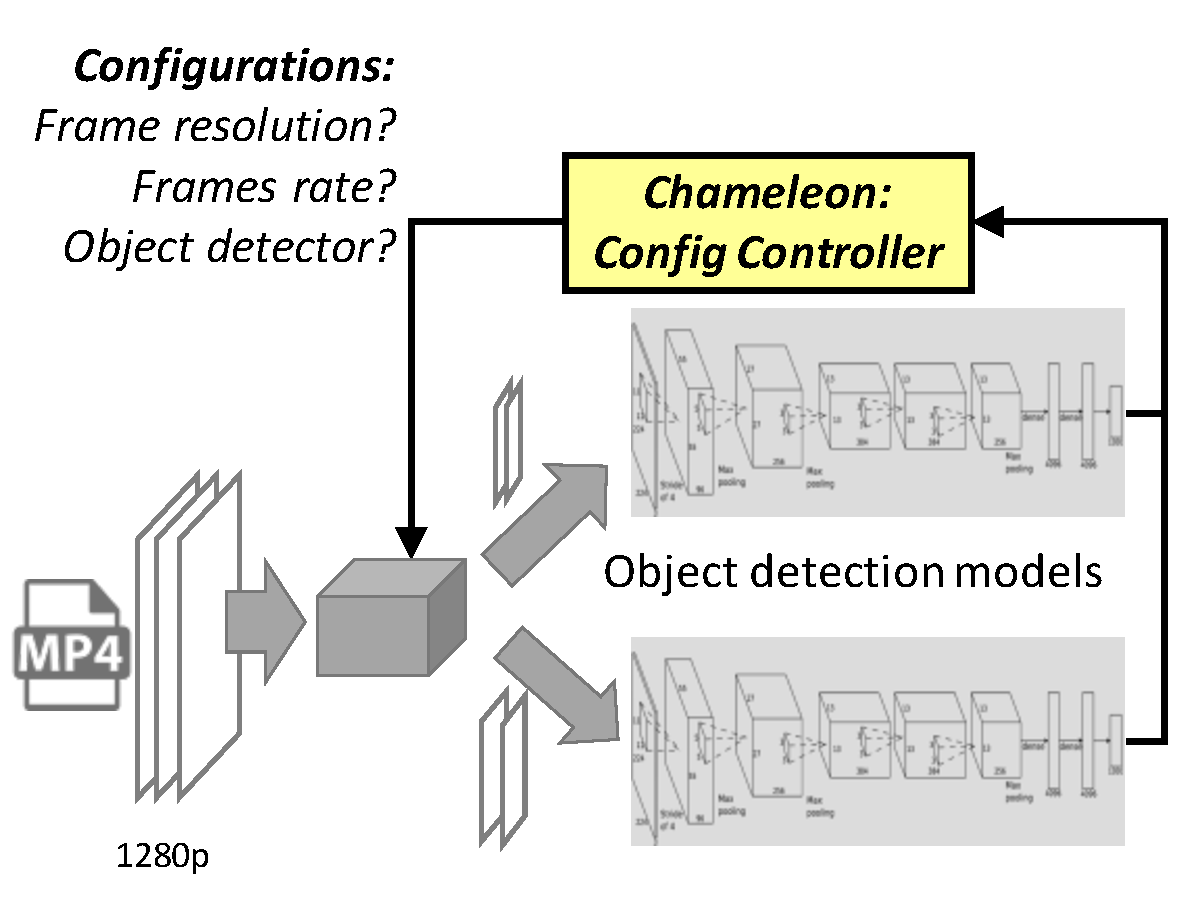
\includegraphics[width=0.25\textwidth]{PaperFigures/PipelineA.pdf}
        \label{subfig:1}
    }
    \subfloat[Pipeline B]
    {
        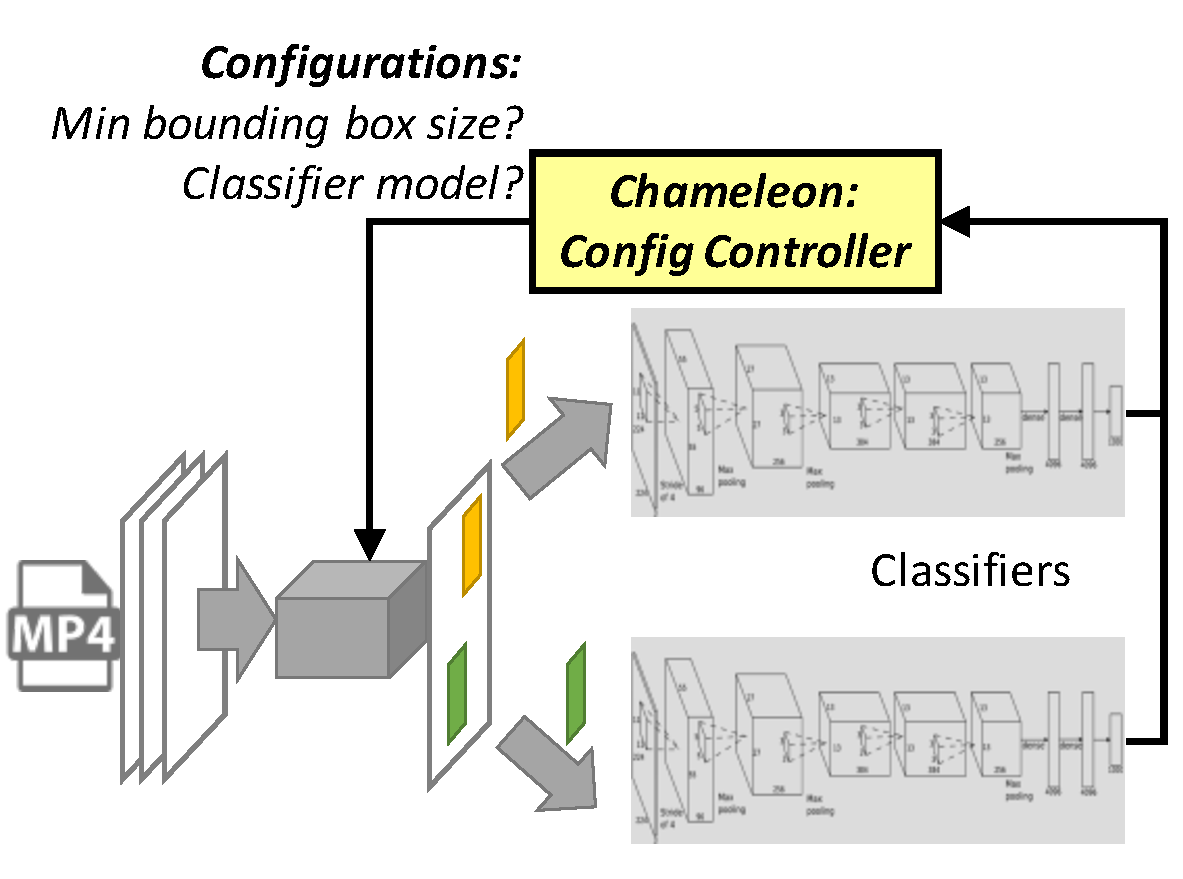
\includegraphics[width=0.25\textwidth]{PaperFigures/PipelineB.pdf}
        \label{subfig:2}
    }
    \caption{\nn-based object detection pipelines and typical configuration
    knobs.}
    \label{fig:pipelines}
\end{figure}

\subsection{Impact of configurations on performance}
\label{subsec:profile}

We now profile the configurations of the object detector pipelines. 
%\mypara{Performance metrics}
The performance of an configuration on a set of frames is 
measured by two metrics: accuracy and cost. 
\begin{packeditemize}
\item {\em Accuracy:} 
We assume that the most expensive configuration---\ie the \emph{golden configuration}---is the most accurate and use it as the ground truth for computing the accuracy of all other configurations, which is consistent with prior work~\cite{videostar,noscope}.
When using configuration $c$, we compute accuracy of a single frame by comparing the detected objects with the objects detected by the golden configuration using the F1 score; \ie the harmonic mean of precision and recall. To compute the accuracy of a frame that was not sampled by $c$, we use the location of objects from the previous sampled frame. 
For a video segment, we compute accuracy as the fraction of frames with F1 score $\geq \alpha$ (most applications care only whether the F1 score is over a threshold).


%We first calculate the F1 score of the configuration's output (a set of 
%labeled bounding boxes) on each frame, and then to capture the F1 score's 
%threshold effect (most applications care only whether the F1 score is over
%a threshold)~\cite{??}, we define accuracy as the fraction of frames whose 
%F1 scores are $\geq \alpha$.
%When calculating the F1 score, we compare against the output of the most expensive 
%configuration, called {\em golden configuration}, as the ground truth, 
%which is consistent with~\cite{videostorm,noscope}.

Note that we identify true positives in the F1 score using two different conditions: 
(1) if the detected bounding box and a ground truth box have the same labels,
and (2) if they have the same labels and have sufficient overlap~\cite{voc}.
The second condition is  stricter than the first; both are useful in real applications.
% Given the output (a set of labeled bounding boxes) of configuration $c$ 
% on frame $x$, we calculate the F1 score
% % , denoted as $f(x,c,c^*)$,
% with respect to the output of the most expensive configuration $c^*$, 
% called {\em golden configuration}
% % . Then the false positives and false 
% % negatives are counted 
% in the same way as prior work in this 
% space~\cite{videostorm,noscope}.
% To capture the accuracy's threshold effect (most applications care
% only if the accuracy is over a threshold)~\cite{??}, we define accuracy 
% of a configuration on a set of frames as the fraction of frames whose 
% F1 scores are over an accuracy threshold $\alpha$.
%, i.e., $\Pr(c(x,c,c^*)>\alpha$.
% the F1 score between
% these  objects and the reference output, those output by the most 
% expensive configuration. 
% We use the standard method
% community~\cite{http://homepages.inf.ed.ac.uk/ckiw/postscript/ijcv_voc09.pdf}
% to map the detected objects and the objects in the reference output, 
% and then calculate the F1 score to report both the precision and 
% the recall. 
\item {\em Cost (resource consumption):}
We use average GPU processing time (with 100\% utilization) per frame
as the metric of resource consumption, because GPU is the dominant resource for the majority of video processing workloads that use NNs.
%GPU resources are much more expensive than other resources like CPU, memory, etc., and hence our focus on their consumption. 
Further, the performance of \nn inference is more dependent on GPU cycles than the typical data analytics task.  %while their demands for other resources are on par.
% Note that if we run more than one configuration on a frame (as in \name), we will count the total GPU time and compute the average accordingly. \ga{Unclear what this means...}
% Specifically, we define the resource consumption as the amount of 
% resources needed by a \nn model to produce inference results on each 
% one second worth of video feed.
\end{packeditemize}
%\mypara{Optimal resource-accuracy tradeoffs}

%Our objective therefore is to maximize the inference accuracy while minimizing the resource consumption. 

%\subsection{Configuration space}



\mypara{Performance impact}
Next, we show how these configurations affect the performance of object
detection.
We use a dataset of 120 clips of traffic videos (the original frame rate and size is 30fps and 960p respectively). The videos are captured by five traffic cameras deployed in diffrent intersections in a metropolitan area.

Figure~\ref{fig:impact-of-configs} shows the impact of various 
configuration knobs in pipeline 
$A$ and $B$ on 
the accuracy and resource consumption.
Different points along the curves represent the resource-accuracy 
tradeoff achieved by setting one knob to different values while 
fixing other knobs to their most expensive values.
We see that one can reduce resource consumption by tuning the values
of these configurations, an observation that has informed 
other work~\cite{videostar}.

At the same time, however, we see that the drop in resource consumption
leads to a substantial accuracy degradation.
This is because, in this experiment, we use a fixed 
configuration for the entire duration of each video (typically lasting
several minutes), which does not adapt to variation in the video content.% \ga{Confusing.}
In the next section, we will show that the relationship between 
configuration and accuracy has great variability over time, so 
dynamically changing the configuration can lead to much better
resource-accuracy tradeoffs.

%\ga{Include graphs for pipeline B too. Include a full scatter plot with all the configurations. Explain the effect of individual knobs, use screen shots if necessary.}




\begin{figure}
    \centering
    \hspace{-0.5cm}
    \subfloat[Frame rate]
    {
        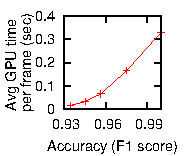
\includegraphics[width=0.18\textwidth]{PaperGraphs/ImpactOfConfig_Sampling.pdf}
        \label{subfig:1}
    }\hspace{-0.7cm}
    \subfloat[Image size]
    {
        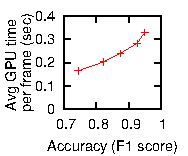
\includegraphics[width=0.18\textwidth]{PaperGraphs/ImpactOfConfig_Size.pdf}
        \label{subfig:2}
    }\hspace{-0.7cm}
    \subfloat[Detection model]
    {
        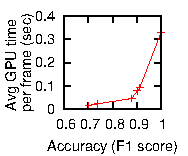
\includegraphics[width=0.18\textwidth]{PaperGraphs/ImpactOfConfig_Detector.pdf}
        \label{subfig:2}
    }\\
    \subfloat[Min size of region of objects]
    {
        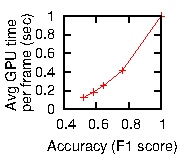
\includegraphics[width=0.18\textwidth]{PaperGraphs/ImpactOfConfig_Classifier_MinArea.pdf}
        \label{subfig:2}
    }\hspace{-0.7cm}
    \subfloat[Classifier]
    {
        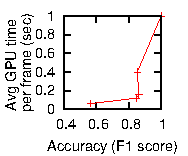
\includegraphics[width=0.18\textwidth]{PaperGraphs/ImpactOfConfig_Classifier_Classifier.pdf}
        \label{subfig:2}
    }
    \caption{Impact of various configuration knobs on the resource-accuracy tradeoffs. The accuracy threshold is $\alpha=0.8$, and the values of each knob are:
    (a) Frame rates: \{30, 10, 5, 2, 1\}fps, 
    (b) Image sizes: \{960, 840, 720, 600, 480\}p, 
    (c) Detection models: Faster RCNN+\{Inception\_ResNet, ResNet101, ResNet50, InceptionV2\}, SSD+\{InceptionV2, MobileNetV1\},
    (d) Minimal area size: 0.5\%, 0.1\%, 0.05\%, 0.01\%,
    (c) Classifier: ResNet101, ResNet50, InceptionV2, MobileNetV1}
    \label{fig:impact-of-configs}
\end{figure}



% prior work has shown that we could strike a 
% favorable balance between accuracy and resource consumption by 
% picking suitable values for key configurations of running 
% \nn~\cite{videostorm,noscope}.
% For instance, Figure~\ref{fig:example} shows the accuracy and 
% resource consumption (in terms of GPU utilization) of using various 
% frame rates on the same video clip. 
%  You can see that while the highest accuracy is achieved at the 
% highest frame rate (highest resource consumption), there is a 
% sweet-spot where a near-optimal accuracy (e.g., \fillme) can be 
% achieved by a \fillme\% lower frame rate.




